\chapter{Les aimants moléculaires}
\section{Définition}

Un molécule, pour recevoir le qualificatif d'aimant, doit remplir deux critères. Tout d'abord, elle doit posséder un moment magnétique. Celui-ci résulte, en général, de l'interaction entre plusieurs centres magnétiques et donne lieux à un configuration où la résultante des moments magnétiques des différents centres est non nulle. 

Il faut en outre que ce moment magnétique ait une orientation préférentielle, le long de laquelle il va venir s'aligner. Les deux directions associées à cette orientation représente les deux configuration d'énergie minimale séparé par une barrière de potentiel. Afin qu'un aimant moléculaire conserve ses propriétés, il faut que l'énergie associé à l'agitation thermique soit plus faible que cette barrière. Dans le cas contraire, la température suffit à retourner aléatoirement le moment magnétique.

Certains aimants moléculaire, en plus de l'axe facile, possèdent également un plan difficile dans lequel l'énergie du moment magnétique est la plus grande. Cela donne naissance à une physique beaucoup plus riche de part l'apparition de phénomènes quantiques tels que le retournement de l'aimantation par effet tunnel~(QTM) ou bien encore la phase de Berry, que nous détaillerons dans la suite.

Malgré ces restrictions, la zoologie des aimants moléculaires est plutôt riche avec des moments magnétique allant de un à plusieurs dizaines $\mu_B$.


\section{Propriétés}
Les aimants moléculaires possèdent de nombreuses propriétés susceptibles de les rendre indispensable aux dispositifs électroniques de demain. Leur taille tout d'abord, en deçà des techniques lithographique, permettrait d'augmenter les densités de stockage, chaque molécule codant une information à travers l'orientation de son moment magnétique. Un telle application est notamment motivé par le faible taux de relaxation, de l'ordre de quelques années en dessous de $2\,K$, qui permettrait d'en faire des éléments de stockage de l'information fiable.

De plus, certains aimant moléculaires peuvent être sensible à un stimulus extérieur tels que la température, la lumières, la pression, un champ électrique ou magnétique ou bien encore un déplacement de charge. Ils peuvent ainsi osciller entre deux configurations magnétiques différentes : "haut spin" et "bas spin". Ces interrupteurs moléculaires pourraient également constituer le composant élémentaires des mémoires de demain.

Les aimants moléculaires peuvent également jouer un rôle non négligeable dans l'information quantique. Cette dernière vise à utiliser les propriétés des systèmes quantiques afin d'obtenir des algorithmes plus efficaces pour la factorisation des nombres premiers~(avec des applications dans la cryptographie notamment) ou bien encore la recherche dans les bases de données. Des phénomènes quantiques tels le QTM ou bien la phase de Berry pourrait être utilisé dans ce cadre.

Nous allons maintenant illustrer certaines de ces propriétés à travers l'exemple d'un aimant moléculaire bien connu le octanuclear fer(III) oxo-hydroxo cluster dont la formule est [Fe$_8$O$_2$(OH)$_{12}$(tacn)$_6$]$^{8+}$ ou Fe$_8$.

\section{L'exemple du Fe$_8$}

\begin{figure}
\centering 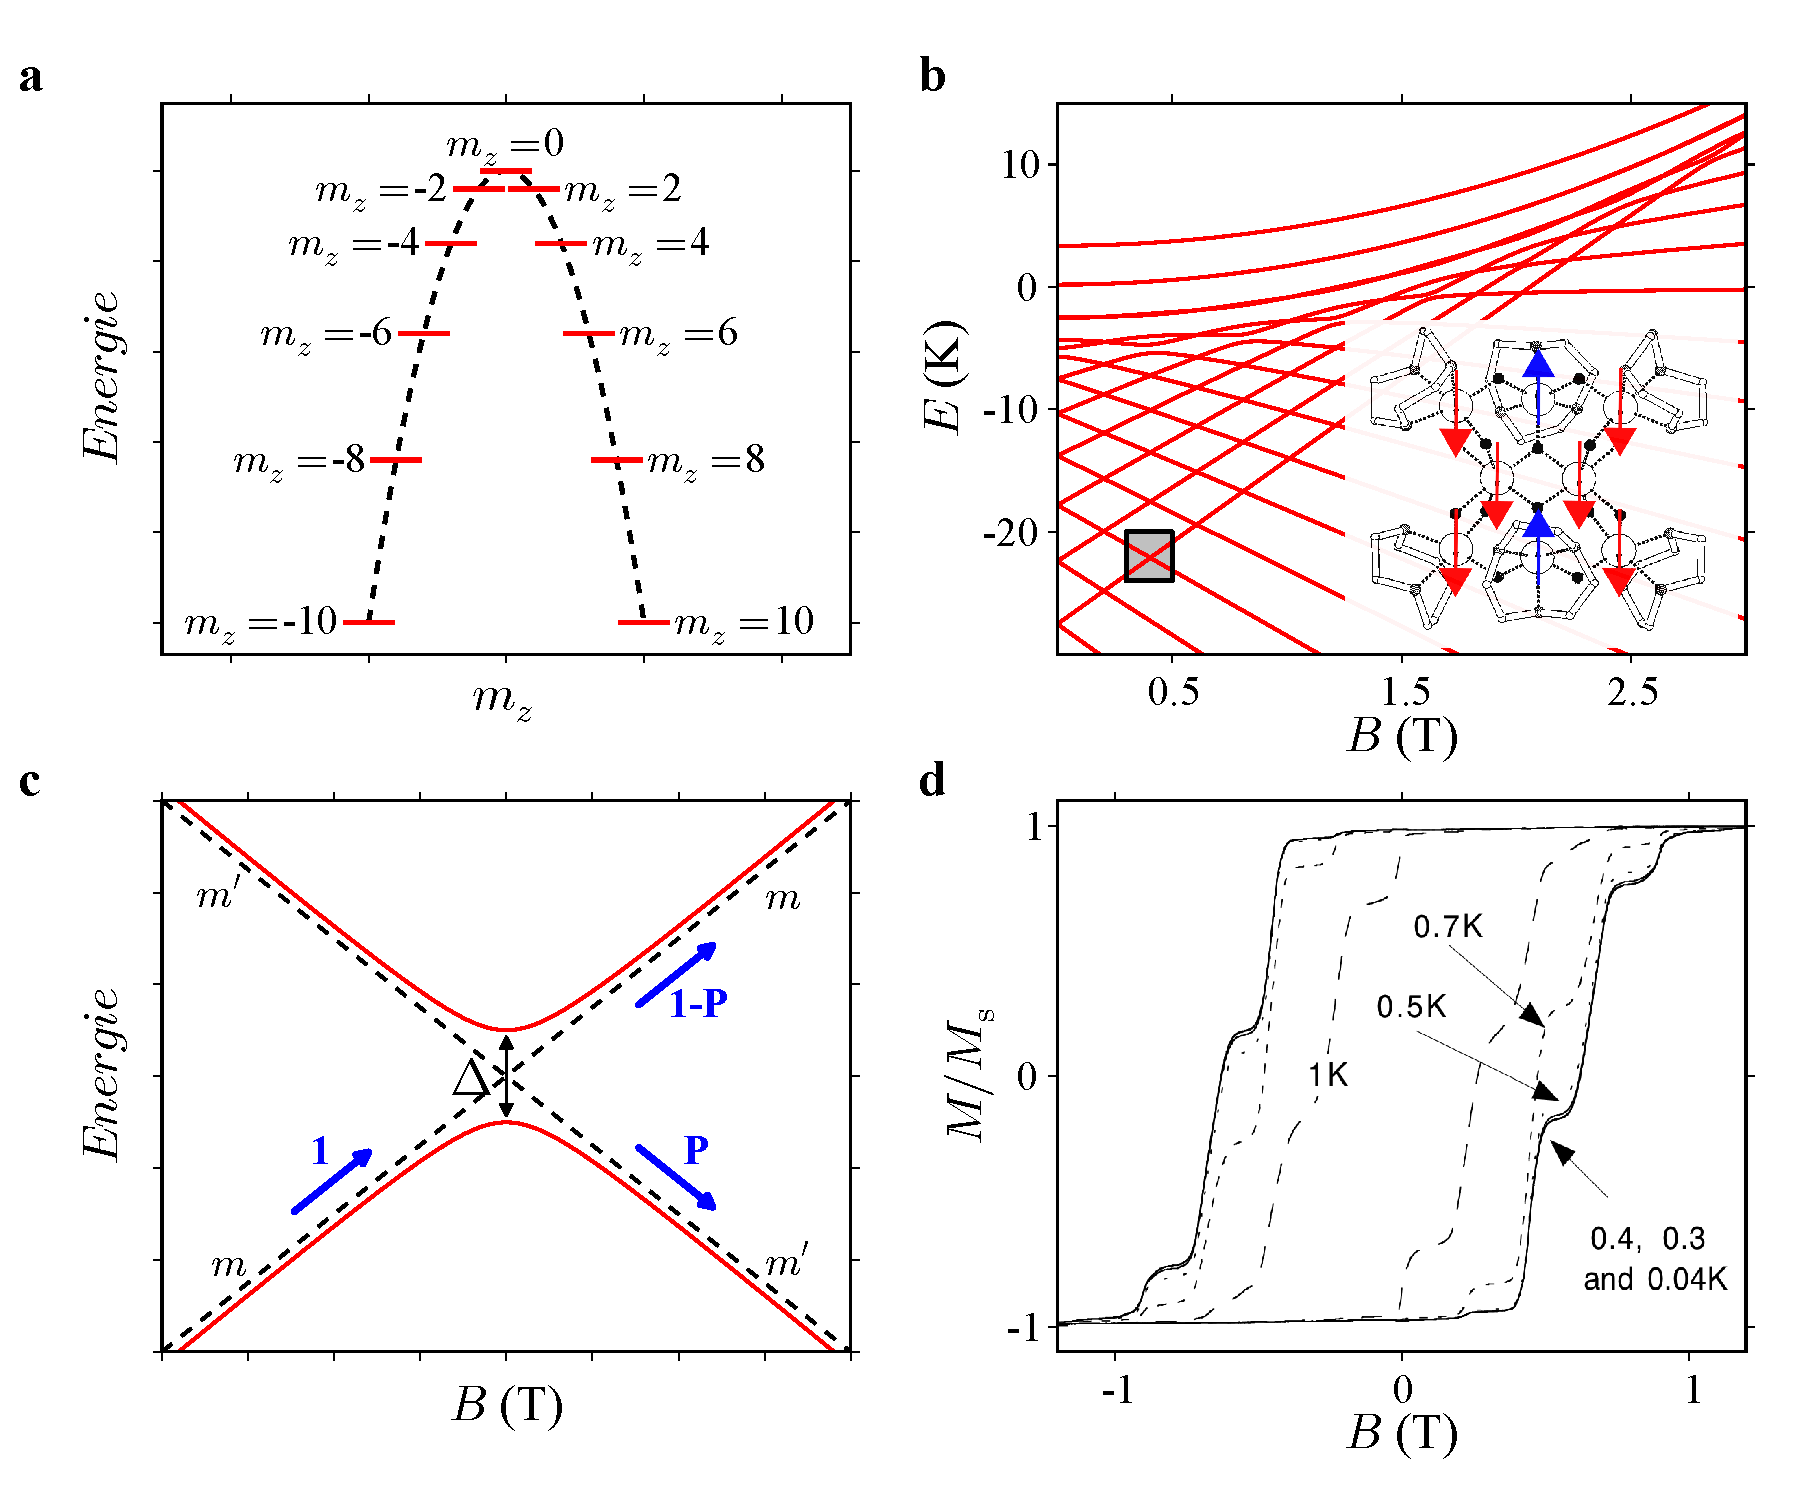
\includegraphics[scale=0.45]{Annexe1/FigureFe8/FigureFe8.pdf} 
\caption{\textbf{a} : énergie en fonction du nombre quantique $m_z$. Les deux orientations $m_z=\pm 10$ sont séparées par une barrière d'énergie de hauteur $|D|S^2$~\cite{Bogani2008}. \textbf{b} : diagramme Zeeman de la molécule Fe$_8$ représentant l'énergie des différents états du système en fonction du champ magnétique. Certains croisements, comme celui marqué d'un carré, sont en fait des anti-croisements traduisant un couplage entre les états. \textbf{c} : anti-croisement représentant un couplage entre les états $m$ et $m'$. \textbf{P} est la probabilité de transition entre les états $m$ et $m'$ lorsque l'on balaie l'anti-croisement en champ magnétique. \textbf{c} : mesure de l'aimantation d'un cristal de Fe$_8$ obtenue par technique micro-squid pour différentes températures. Les anti-croisements sont visibles à travers les marches qui traduisent un renversement de l'aimantation d'un grand nombre de molécules pour des valeurs particulières du champ magnétique~(extrait de \cite{MagGoesNano}).}
\label{Fe8Zeeman}
\end{figure}


Le Fe$_8$ se compose de huit atomes de fer de degré d'oxydation III, chacun de ces atomes constituant un centre magnétique de spin 5/2. De part les différentes interactions qui les lient, ils adoptent la configuration présenté dans la Fig.\ref{Fe8Zeeman}.\textbf{b} en encart avec un moment résultant total de $S=10$, le moment magnétique des deux atomes centraux se trouvant dans la direction opposée aux six atomes latéraux.

Les propriété magnétique de ce système peuvent \^etre décrite par l'hamiltonien suivant :
\begin{eqnarray}
H =  -DS_z^2 + \frac{E}{2} ( S_+^2  + S_-^2) + g\mu_b B S_z 
\end{eqnarray}
où $D$ est le paramètre d'anisotropie axiale, $E$ est le paramètre d'anysotropie transversale, $S_z$ et la projection sur $z$ du moment magnétique et $S_+$ et $S_-$ les opérateurs création anhilation.

A champ magnétique nul, les différents états magnétiques de la molécule se trouvent de part et d'autre d'un puit de potentiel, les deux états de plus basses énergie, $m_z=\pm10$ étant séparé par une énergie $D|S|^2$ où $S$ est le moment magnétique de la molécule (cf Fig.\ref{Fe8Zeeman}.\textbf{a}). Si l'énergie associé à l'agitation thermique est telle que $k_BT \ll D|S|^2$, l'aimantation de la molécule est parfaitement définie et aligné le long de l'axe $z$. Elle peut alors avoir deux orientation : \textit{up} lorsque $m_z=+10$ et \textit{down} lorsque $m_z=-10$.

Lorsque l'on applique un champ magnétique, l'énergie associée aux différents états du système va évoluer. On peut représenter cette évolution à l'aide d'un diagramme Zeeman dans lequel on représente l'énergie de chaque niveau en fonction du champ magnétique. La Fig.\ref{Fe8Zeeman}.\textbf{b} présente le digramme Zeeman associé au Fe$_8$ pour un champ magnétique allant jusqu'à $3\,T$. Un tel diagramme comporte de nombreux croisements pour lesquels deux états du système sont dégénérés.

Cependant, la présence d'un plan difficile introduit un couplage entre certains états du système. Quand ceux-ci sont en résonance~(i.e. ont la m\^eme énergie), le couplage est maximal, ce qui se traduit dans le diagramme Zeeman par ce que l'on appelle un anti-croisement. C'est notamment le cas de l'anti-croisement repéré par un rectangle dans la Fig.\ref{Fe8Zeeman}.\textbf{b}. La Fig.\ref{Fe8Zeeman}.\textbf{c} propose une vision schématique de ce dernier où $m$ et $m'$ sont les états du système loin de la résonance, $\Delta$ désigne la séparation en énergie entre les deux états et la ligne pointillé représente le diagramme Zeeman en l'absence de plan difficile.

Lorsque l'on balaie le champ magnétique autour d'un tel anti-croisement, il y a une certaine probabilité de passer de l'état $m$ à l'état $m'$ et vice-versas. Cette probabilité est régie par la formule de Landau-Zener~\cite{Zener1932} qui dépend à la fois de la séparation minimale entre les deux niveaux~$\Delta$, ainsi que de la vitesse de balayage du champ magnétique~$\frac{dB_z}{dt}$. Cette probabilité peut s'exprimer de la façon suivante :
\begin{eqnarray}
P = 1 - \exp \left( -\frac{\pi \Delta^2}{2 \hbar g \mu_B |m-m'|\frac{dB_z}{dt}} \right)
\end{eqnarray}
ou P est la probabilité de passer de l'état $m$ à l'état $m'$. On constate tout d'abord que si la vitesse est très faible, la probabilité de passer d'un état à l'autre tend vers 1. On retrouve ici le théorème adiabatique. A l'autre bout de l'échelle, si je balaie très rapidement le champ magnétique cette probabilité tend vers zéro. Tout se passe comme si le système n'avait pas eu le temps de "sentir" l'anti-croisement.


C'est lorsque le champ magnétique balaie un anti-croisement que le phénomène de QTM pourra être observé. En effet, le système pourra alors passé d'un coté de la barrière sans avoir à fournir l'énergie correspondante. Autrement dit, le renversement va se faire par effet tunnel à travers la barrière le potentiel, d'où le nom de renversement de l'aimantation par effet tunnel~(Qantum Tunneling of the Magnetization ou QTM en anglais).

Ce phénomène quantique peut être mise en évidence par une mesure de l'aimantation d'une assemblé de molécule. Une telle mesure consiste à relever l'aimantation d'un cristal moléculaire en fonction du champ magnétique. L'aimantation du cristal est d'abord amenée à saturation par l'application d'un fort champ magnétique. Celui-ci est ensuite balayé jusqu'à obtenir la saturation du cristal dans la direction opposée. Lorsque l'aimantation des molécules composant le cristal se retourne, elles modifient les lignes de champ environnante. De telle variation peuvent \^etre mesuré par une technique de micro-SQUID. La Fig.\ref{Fe8Zeeman}.\textbf{d} présente la mesure de l'aimantation d'un cristal de Fe$_8$ pour différentes températures et pour une vitesse de balayage de $14\,mT.s^{-1}$.

La courbe montre une série de marches qui sont d\^ues au retournement par QTM. Chacune d'elles correspond à un anti-croisement sur lequel l'aimantation à une probabilité élevée de transiter. Lorsque l'on diminue la température, le taux de retournement diminue car les transitions assistées thermiquement diminuent. Cette courbe devient indépendante de la température au dessous de 400\,mK et on observe les transitions correspondantes aux niveaux de plus basse énergie. 
